\documentclass[11pt]{article}
\usepackage[utf8]{inputenc}
\usepackage{graphicx}
\usepackage{booktabs}
\usepackage{array}
\usepackage{tikz}

\title{Test Document 3: Tables and Figures}
\author{Graphics Test}
\date{\today}

\begin{document}

\maketitle

\section{Introduction}
This document demonstrates tables and figures in LaTeX.

\section{Tables}

\subsection{Simple Table}
\begin{table}[h]
\centering
\caption{Sample Data Table}
\begin{tabular}{@{}lrr@{}}
\toprule
Item & Quantity & Price (\$) \\
\midrule
Apples & 10 & 5.50 \\
Oranges & 15 & 8.25 \\
Bananas & 20 & 6.00 \\
\bottomrule
\end{tabular}
\end{table}

\subsection{Complex Table}
\begin{table}[h]
\centering
\caption{Performance Metrics}
\begin{tabular}{|l|c|c|c|}
\hline
\textbf{Algorithm} & \textbf{Speed (ms)} & \textbf{Accuracy (\%)} & \textbf{Memory (MB)} \\
\hline
Method A & 125 & 95.2 & 512 \\
\hline
Method B & 89 & 97.8 & 768 \\
\hline
Method C & 156 & 93.1 & 384 \\
\hline
\end{tabular}
\end{table}

\section{Figures}

\subsection{TikZ Drawing}
\begin{figure}[h]
\centering
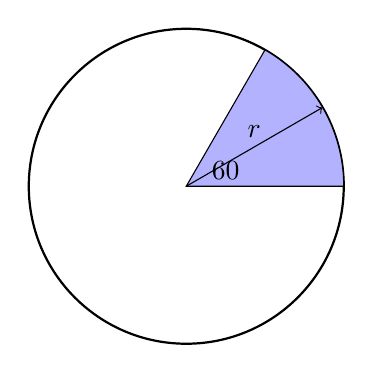
\begin{tikzpicture}
    \draw[thick] (0,0) circle (2cm);
    \draw[fill=blue!30] (0,0) -- (2,0) arc (0:60:2cm) -- cycle;
    \draw[->] (0,0) -- (1.73,1) node[midway,above] {$r$};
    \node at (0.5,0.2) {$60°$};
\end{tikzpicture}
\caption{A simple geometric figure created with TikZ}
\end{figure}

\subsection{Another TikZ Example}
\begin{figure}[h]
\centering
\begin{tikzpicture}[scale=0.8]
    \draw[step=1cm,gray,very thin] (-2,-2) grid (4,4);
    \draw[thick,->] (-2,0) -- (4.5,0) node[anchor=north west] {x};
    \draw[thick,->] (0,-2) -- (0,4.5) node[anchor=south east] {y};
    \draw[color=red,thick] plot (\x,{0.5*\x*\x - 2}) node[right] {$f(x) = \frac{x^2}{2} - 2$};
\end{tikzpicture}
\caption{Function plot using TikZ}
\end{figure}

\end{document}